
\section{Foundations of Probability}

\subsection{Principle Definitions}
Some terms that are needed to build the foundations are defined below.
\begin{itemize}
    \item \textbf{Sample space} S is a set that includes all possible outcomes of a random experiment listed in a mutually exclusive and exhaustive way.
    \item \textbf{Mutually exclusive} means that outcomes of the set do not overlap.
    \item \textbf{Exhaustive} means that the list contains all possible outcomes.
    \item \textbf{Event} is a set of outcomes that is a subset of the sample space.
\end{itemize}

\subsection{Venn Diagrams and Set Theory}

\begin{figure}[!hbtp]
    \centering
    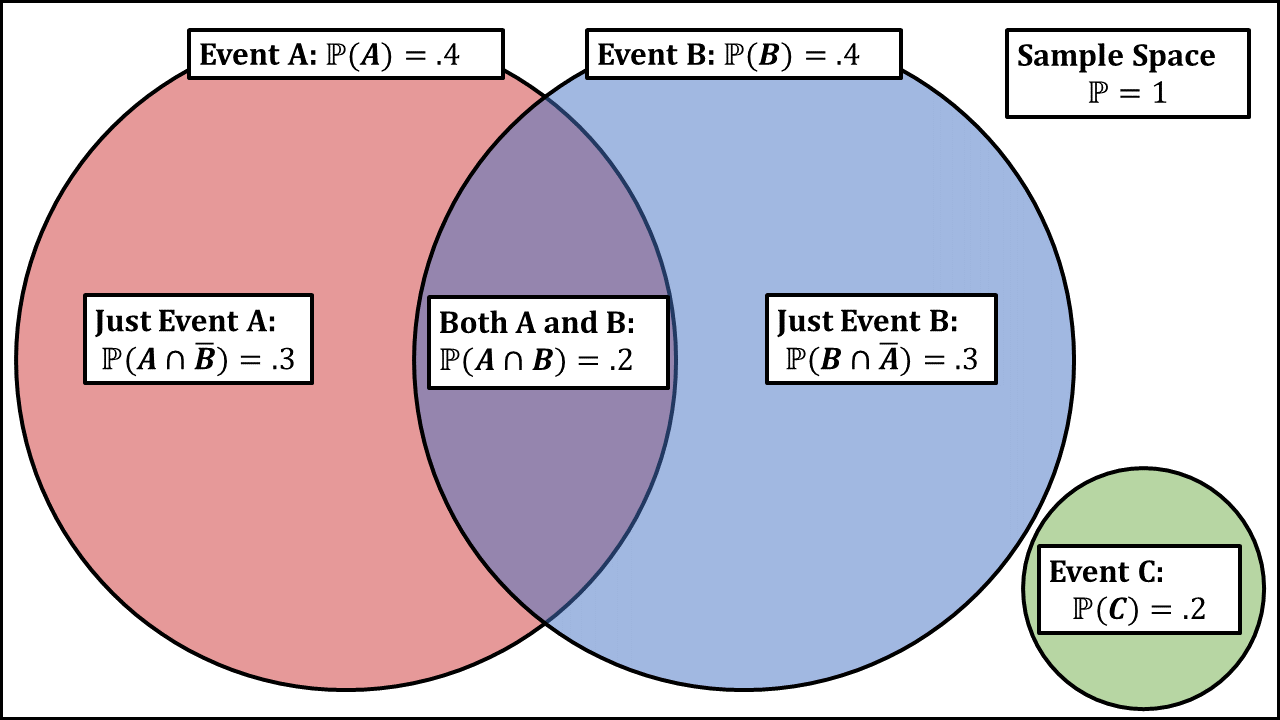
\includegraphics[scale=.3]{Images/venndiagram.PNG}
    \caption{An example of a sample space being represented by a venn diagram.}
    \label{fig:venndiagram}
\end{figure}